% Equivalence classes of "has the same square" on a small set.
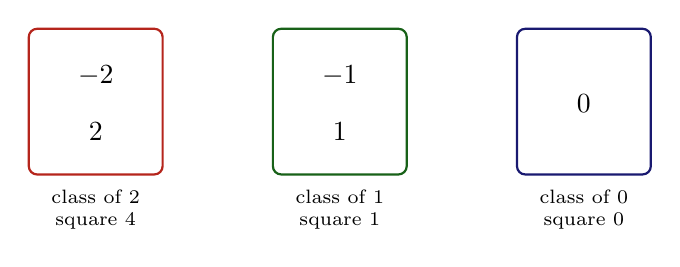
\begin{tikzpicture}[x=1cm,y=1cm]
  \draw[BrickRed,thick,rounded corners=3pt] (0,0) rectangle (1.7,1.85);
  \node at (0.85,1.25) {$-2$};
  \node at (0.85,0.55) {$2$};
  \node[font=\scriptsize,text=black,align=center] at (0.85,-0.45) {class of $2$\\square $4$};

  \draw[ForestGreen!70!black,thick,rounded corners=3pt] (3.1,0) rectangle (4.8,1.85);
  \node at (3.95,1.25) {$-1$};
  \node at (3.95,0.55) {$1$};
  \node[font=\scriptsize,text=black,align=center] at (3.95,-0.45) {class of $1$\\square $1$};

  \draw[MidnightBlue,thick,rounded corners=3pt] (6.2,0) rectangle (7.9,1.85);
  \node at (7.05,0.9) {$0$};
  \node[font=\scriptsize,text=black,align=center] at (7.05,-0.45) {class of $0$\\square $0$};
\end{tikzpicture}
